\subsection{Principes de conception d'UI et règles ergonomiques}
\label{sec:chap2:3:2}
Les principes de conceptions présentés dans la section précédente constitue des recommandations de haut niveau difficilement applicable de manière formelle. Ce paragraphe permet de faire le lien entre les guidelines d'une part  et les règles ergonomiques formelle d'autre part. Dans le cadre de la migration les règles ergonomiques formelles seront utilisées par le processus pour adapter l'UI de départ à la table interactive d'arrivée. Une approche de dérivation des règles ergonomiques formelles et utilisables est proposée par Vanderdonckt \citep{Vanderdonckt1997} dans son processus de conception automatique d'UI.

\subsubsection{Processus de conception automatique de Vanderdonckt}
\begin{figure}[ht]
\begin{center}
\caption{Conception automatique de l'UI}
\label{fig:15}
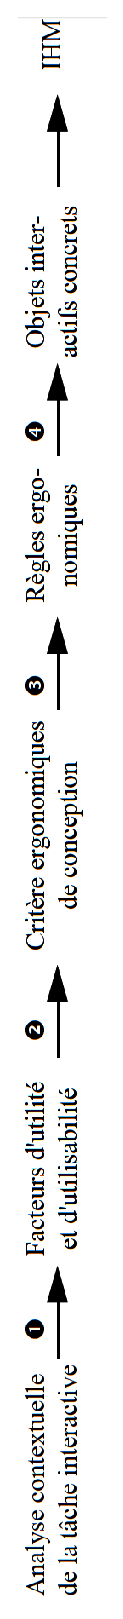
\includegraphics[angle=270,scale=.55]{chap2/img-15.eps} 
\end{center}\end{figure}
Ce processus a pour but de proposer une approche de conception qui assiste les concepteurs et qui prend en compte les critères ergonomiques. Dans un contexte définie, la démarche de conception de l'UI peut être automatisée en quatre phases suivantes (cf. figure \ref{fig:15}):
\begin{enumerate}
\item dériver systématiquement les facteurs d'utilité et d'utilisabilité que l'IHM doit satisfaire, à partir des paramètres décrivant la tâche interactive, les utilisateurs, l'environnement physique issus d'une analyse de la tâche;
\item dériver systématiquement une pondération de critères ergonomiques de conception
appropriés à la tâche interactive, à partir des facteurs retenus;
\item dériver systématiquement un sous-ensemble de règles ergonomiques non
conflictuelles en les extrayant d'un corpus ergonomicus ; ces règles sont censées respecter chacune des critères, être complètes et cohérentes, à partir des critères dégagés;
\item générer automatiquement les objets interactifs concrets de la présentation
de l'IHM sur base de modèles (p. ex. le modèle de structuration des informations), à partir des règles ergonomiques dérivées.
\end{enumerate}
Dans le cadre de la migration d'UI vers une table interactive, l'objectif est d'adapter une UI existante. Pour la génération des objets interactifs concrets pour une table interactive donnée, il est indispensable d'identifier l'ensemble des règles ergonomiques pour différents étapes de la migration. Les règles ergonomiques sont dérivées à partir des critères ergonomiques de conception pondérés en fonction des facteurs d'utilités et d'utilisabilités de la plateforme.  Les critères ergonomiques de conception varient en nombre, en forme et en couverture (p. ex. les critères de Scapin[Bastien and Scapin 1995], les heuristiques de Nielsen[Nielsen and Molich 1990]).

En considérant les huit critères ergonomiques de conception d'UI de Scapin (la compatibilité, l'homogénéité, la concision, la flexibilité, le feed-back et le guidage, la charge informationnelle, le contrôle explicite et la gestion des erreurs), les principes de conception décrite à ci-dessus(cf. section \ref{sec:chap2:3:1}) permettent de respecter certains critères ergonomiques de conception. Les principes de conception permettant de décrire une UI collaborative pour une table interactive (cf. section \ref{sec:chap2:3:1:2}) sont conforment au guidage. En effet ils rendent accessibles des éléments d'une tâche à chaque utilisateur autour de la table, ce qui est une forme de guidage pour accomplir une tâche. La capacité des éléments de l'UI à s'adapter aux nombre d'utilisateurs. Tous ces principes de conception de la section seront utilisés pour adapter les UI à la table interactive et aux utilisateurs finaux, ils sont donc conformes au critère ergonomique de conception flexibilité.


\subsection{Des principes de conception d'UI aux règles ergonomiques pour la migration}
Les principes de conception vont des expressions de haut niveau aux cas de bas niveau qui sont limités à des familles de cas spécifiques[C Stephanidis and D Akoumianakis 1999; Ohnemus 1997]. Les rôles des principes de conception est de guider les différents choix effectuer durant le processus de développement[Mariage, Vanderdonckt, and Pribeanu 2004]. Tout comme les facteurs d'utilisabilité et les critères ergonomiques qui en découlent, les principes de conception peuvent être raffinés en règles ergonomiques qui guideront la génération de l'UI de la table interactive.  
La traduction des principes de haut niveau en règles ergonomiques utilisables pendant la migration soulève plusieurs problématiques: 
\begin{enumerate}
\item quels rôles effectifs pour ces règles formalisées pendant la migration? En effet pour la conception automatique [Vanderdonckt 1997], ces règles permettent de sélectionner, placer et éditer manuellement les objets interactif concrets.
\item Comment formalisés les règles ergonomiques de la migration pour les rendre opérationnelles? Dans le cadre de la conception, il existe plusieurs formalisation.Par exemple Denley \textit{et al.} formalisent les règles ergonomiques au moyen de l'équation 
\begin{equation}
X=f\left( T,U,C,P_s\right) \Longrightarrow Y parce\ que R=\left( Y=\left( f\left( X\right) \right) \right)\\
avec\ garantie\ \textit{p} >seuil 
\end{equation}

où X=ensemble des attributs de déclenchement\\
T = ensemble des attributs propres à la tâche interactive\\
U = ensemble des attributs propres à l'utilisateur\\
C = ensemble des attributs propres à l'environnement physique\\
Ps = performance souhaitée\\
Y = prescription\\
R = raison\\
\end{enumerate}

